\documentclass[10pt,twocolumn,letterpaper]{article}
\usepackage{cvpr}
\usepackage{times}
\usepackage{graphicx}
\usepackage{amsmath,amssymb}
\usepackage[utf8]{inputenc}
\usepackage{url}
\usepackage{hyperref}
\usepackage{booktabs}
\usepackage{enumitem}
\usepackage{tikz}
\usetikzlibrary{shapes,arrows,arrows.meta,positioning,fit,backgrounds,calc}
\usepackage{xcolor}
\usepackage{tcolorbox}
\tcbuselibrary{skins,breakable}

\setlength{\columnsep}{0.2in}
\setlength{\parindent}{1.5em}
\setlength{\parskip}{0pt}
\usepackage{indentfirst}

% Compact title spacing
\makeatletter
\def\@maketitle{%
  \newpage
  \null
  \vskip -0.4in
  \begin{center}%
    {\Large\bfseries \@title \par}%
    \vskip 0.3em%
    {\large
      \lineskip .4em%
      \begin{tabular}[t]{c}%
        \@author
      \end{tabular}\par}%
  \end{center}%
  \par
  \vskip 0.2em}
\makeatother

% Tighter section spacing
\makeatletter
\renewcommand\section{\@startsection{section}{1}{\z@}%
  {5pt plus 2pt minus 2pt}{3pt plus 1pt minus 0pt}%
  {\large\bfseries}}
\renewcommand\subsection{\@startsection{subsection}{2}{\z@}%
  {4pt plus 2pt minus 1pt}{2pt plus 1pt minus 0pt}%
  {\normalsize\bfseries}}
\makeatother

% Case box for qualitative examples
\newtcolorbox{casebox}[1][]{
  colback=gray!5, colframe=gray!60, boxrule=0.4pt, arc=1pt,
  left=4pt, right=4pt, top=2pt, bottom=2pt,
  fontupper=\footnotesize, breakable, #1
}

\begin{document}

\title{An Agentic RAG System for Medical Literature Question Answering}
\author{Ruoyu Zhang \quad Xu Chen\\
Auburn University, Auburn, AL, USA\\
{\tt\small \{ruz0002, xzc0066\}@auburn.edu}
}
\maketitle

\vspace{-2pt}
\section{Abstract}

We present a clinical Retrieval-Augmented Generation (RAG) agent that answers USMLE-style medical questions grounded in authoritative textbook knowledge. Built on a LangGraph-based two-level agentic architecture, the system ingests 340K+ text chunks from 18 medical textbooks and employs hybrid retrieval (dense semantic search plus BM25 sparse matching) with cross-encoder reranking, hierarchical parent-child chunking, and token-aware context compression to produce source-attributed answers. Unlike fixed single-pass RAG pipelines, our agent dynamically decomposes complex queries into sub-questions, plans retrieval strategies at each step, and compresses accumulated evidence to stay within token budgets while preserving clinical facts. Evaluated on 100 questions from the MedQA benchmark, the system achieves 80\% overall accuracy and 86\% source attribution rate after three rounds of iterative optimization, improving from an initial 65\% accuracy while simultaneously reducing average latency from 32.1s to 26.0s per question. We analyze the system along three safety-critical dimensions---in-knowledge-base accuracy, source grounding fidelity, and out-of-knowledge-base boundary awareness---and present qualitative case studies demonstrating both successful multi-step clinical reasoning (e.g., diagnosing cholesterol embolization from a multi-organ clinical vignette) and characteristic failure modes (over-confident answers on out-of-knowledge topics, outdated guidelines in the corpus). Our work illustrates that agentic RAG can substantially outperform naive retrieval baselines in medical QA, while also revealing concrete limitations that must be addressed for deployment in safety-critical clinical workflows.

\section{Introduction}

Medical question answering requires both broad domain knowledge and precise clinical reasoning. Large language models (LLMs) have demonstrated remarkable general-purpose capabilities, yet they remain prone to hallucination in high-stakes medical domains where factual accuracy is critical~\cite{ji2023survey}. Retrieval-Augmented Generation (RAG)~\cite{lewis2020retrieval} addresses this limitation by grounding LLM outputs in retrieved evidence, but standard single-pass RAG pipelines lack the ability to iteratively refine their retrieval strategy based on intermediate results.

This project builds an \textbf{agentic RAG system} for medical literature question answering. The key insight is that medical questions often require multi-step reasoning: identifying the relevant clinical domain, retrieving evidence from multiple sources, reasoning over partial evidence, and synthesizing a grounded answer with proper source attribution. Our system implements this through a LangGraph~\cite{langgraph} workflow where an LLM-based orchestrator dynamically decides \emph{when} to search, \emph{what} to search for, and \emph{when} sufficient evidence has been gathered.

\textbf{Contributions.}
(1)~We design and implement a two-level LangGraph agent with query decomposition, hybrid retrieval with cross-encoder reranking, hierarchical parent-child chunking, and token-aware context compression.
(2)~We evaluate on 100 USMLE-style questions from MedQA~\cite{jin2021disease} along three safety-critical dimensions: in-KB accuracy, source grounding, and out-of-KB boundary awareness.
(3)~We document the iterative optimization process that improved accuracy from 65\% to 80\% while reducing per-question latency by 19\%.
(4)~We provide qualitative case studies illustrating both successful reasoning chains and characteristic failure modes.

\section{Background and Related Work}

\subsection{Retrieval-Augmented Generation}

RAG~\cite{lewis2020retrieval} augments language model generation with retrieved passages from an external knowledge base, enabling the model to produce answers grounded in factual evidence rather than relying solely on parametric knowledge. The original RAG formulation treats retrieval as a single step conditioning generation. \textbf{Relevance to our work:} We extend this paradigm in two directions: (i)~we replace the single-retrieval-step assumption with an \emph{agentic loop} where retrieval can be issued multiple times based on intermediate reasoning, and (ii)~we enforce strict source attribution for every factual claim, treating RAG not only as an accuracy tool but also as a safety mechanism for medical applications.

Follow-up work on RAG has explored query rewriting~\cite{ma2023query}, multi-hop retrieval~\cite{trivedi2023interleaving}, and self-correcting retrieval~\cite{asai2024selfrag}. Self-RAG~\cite{asai2024selfrag} trains a model with special reflection tokens to decide when to retrieve and whether retrieved passages are relevant. Our work takes a different, prompt-engineered approach: rather than fine-tuning the base model, we rely on structured prompting and a LangGraph control flow to achieve similar reflective behavior in a model-agnostic way. This design decision was motivated by practical constraints (we use a commercial LLM API) and allows us to swap the underlying LLM (Gemini, Ollama local models) without retraining.

\subsection{Medical RAG and Domain-Specific Benchmarks}

\textbf{MedRAG}~\cite{xiong2024benchmarking} provides a systematic benchmark for RAG in medicine, covering five medical QA datasets and four corpora (PubMed, Textbooks, StatPearls, Wikipedia). Their work establishes that retrieval-augmented approaches significantly outperform closed-book LLMs on medical benchmarks, and that corpus choice matters: textbook corpora outperform PubMed abstracts for USMLE-style questions because textbooks cover fundamental clinical knowledge at the appropriate level of abstraction.
\textbf{Relevance to our work:} We adopt MedRAG's Textbooks corpus as our knowledge base, specifically because the MedQA benchmark targets USMLE-style questions that map well to textbook content. However, MedRAG evaluates fixed-pipeline RAG (single retrieval step + generation); we extend this to an agentic setting and report complementary metrics (source attribution rate, refusal rate) that MedRAG does not emphasize.

Other medical RAG systems include Almanac~\cite{zakka2024almanac}, which focuses on curated clinical guidelines and demonstrates the importance of source traceability, and ClinicalGPT variants that incorporate retrieval. Our system aligns with Almanac's emphasis on traceability by requiring source citations for every answer.

\subsection{Agentic Reasoning for LLMs}

\textbf{ReAct}~\cite{yao2023react} interleaves reasoning traces with actions, enabling LLMs to dynamically plan and execute multi-step tasks. \textbf{Relevance to our work:} Our orchestrator node implements a ReAct-style loop in the LangGraph framework: at each iteration the LLM can either emit a tool call (search or retrieve) or produce a final answer. The key extension beyond vanilla ReAct is our token-aware context compression: because medical queries often require 3--8 retrieval rounds and each textbook passage can be several hundred tokens long, naive accumulation of the reasoning history quickly exhausts the context window. Our compression mechanism (\S\ref{sec:compression}) addresses this by periodically summarizing accumulated evidence into a structured clinical note.

\textbf{LangGraph}~\cite{langgraph} provides a stateful graph-based orchestration framework for LLM agents, with first-class support for conditional routing, parallel execution via \texttt{Send()}, and checkpoint-based memory. We use LangGraph to implement a two-level graph where the top level handles query decomposition and fan-out, while each sub-question is handled by an independent agent subgraph.

\textbf{Relation to tool-using agents.} Recent work on tool-using agents~\cite{schick2023toolformer,qin2023toolllm} has demonstrated that LLMs can be trained or prompted to use external tools. Our system uses the simpler prompted approach, exposing two tools to the LLM: \texttt{search\_child\_chunks} (for semantic+lexical retrieval) and \texttt{retrieve\_parent\_chunks} (for expanding context around a promising passage).

\subsection{Dense-Sparse Hybrid Retrieval and Reranking}

Dense retrievers based on sentence embeddings~\cite{reimers2019sentence,karpukhin2020dense} capture semantic similarity but can miss exact-term matches that are critical in medical contexts (e.g., specific drug names, abbreviations like ``HbA1c''). Conversely, sparse lexical methods like BM25 excel at exact matching but miss paraphrases. Hybrid retrieval combining both has been shown to improve robustness, particularly for domain-specific queries~\cite{lin2021pyserini}. \textbf{Relevance to our work:} We use \texttt{all-mpnet-base-v2}~\cite{reimers2019sentence} for dense embeddings and BM25 for sparse matching, fusing scores via Qdrant's hybrid retrieval mode. This is particularly important for medical queries, where we observed during development that dense-only retrieval frequently missed passages containing exact drug brand names or specific lab values mentioned in the query.

Cross-encoder rerankers~\cite{nogueira2019passage} score query-document pairs jointly, providing higher precision than bi-encoder retrieval at the cost of computational efficiency. Standard practice is to over-fetch candidates with a fast retriever and rerank with a cross-encoder~\cite{khattab2020colbert}. \textbf{Relevance to our work:} Adding \texttt{ms-marco-MiniLM-L-6-v2}~\cite{nogueira2019passage} as a reranker between v1 and v2 of our system was the single largest quality improvement we observed, boosting in-KB accuracy by 13 percentage points (\S\ref{sec:results}).

\subsection{Hierarchical and Parent-Child Chunking}

Fixed-size chunking is the default in most RAG systems, but it creates a tension: small chunks improve retrieval precision but provide insufficient context for the generator, while large chunks hurt retrieval precision. \emph{Parent-child} or \emph{small-to-big} retrieval~\cite{llamaindex2023parent} resolves this by indexing small child chunks for retrieval but returning larger parent chunks for generation. \textbf{Relevance to our work:} We adopt this pattern with a hierarchical splitting strategy that respects document structure (markdown headers). This is particularly important for medical textbooks, which have clear hierarchical section structure (e.g., disease $\to$ clinical features $\to$ diagnosis $\to$ treatment) that is semantically meaningful and worth preserving.

\subsection{MedQA Benchmark}

MedQA~\cite{jin2021disease} is a large-scale, open-domain medical QA dataset derived from professional medical board examinations (primarily USMLE). Each question is multiple-choice with a clinical vignette, requiring both factual recall and multi-step clinical reasoning. \textbf{Relevance to our work:} We evaluate on MedQA because it aligns well with textbook knowledge and is widely used as a benchmark for medical LLMs. Compared to MedMCQA or PubMedQA, MedQA questions require more integrative reasoning (connecting lab findings with clinical presentation), which is where an agentic (rather than single-pass) RAG approach should offer the greatest benefit.

\section{Approach}

Figure~\ref{fig:architecture} provides an overview of our two-level agentic architecture.

\begin{figure}[t]
\centering
\resizebox{\columnwidth}{!}{%
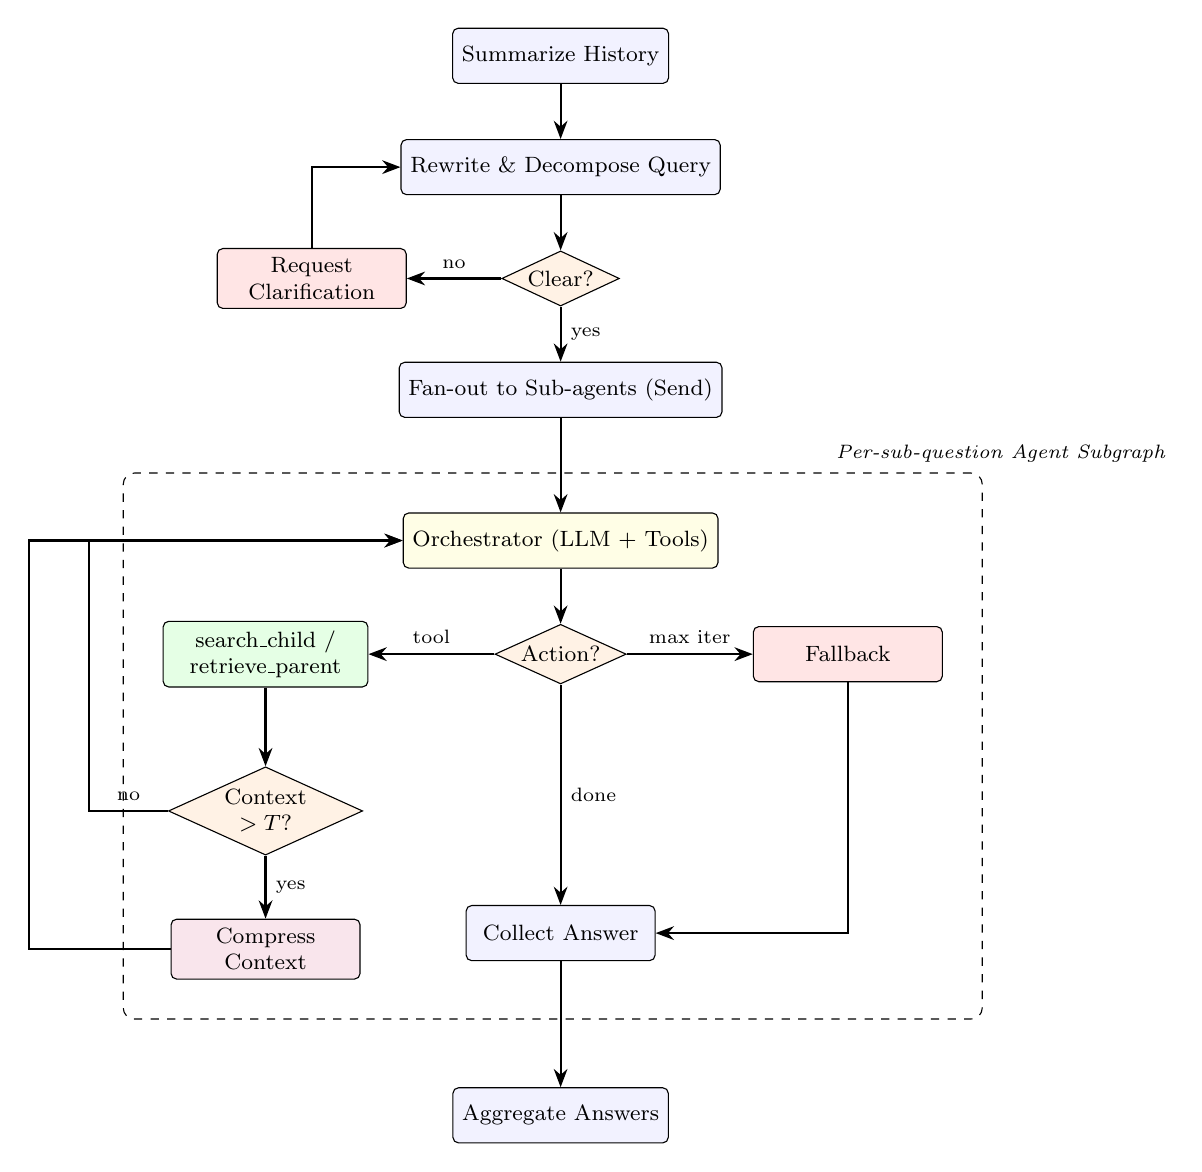
\begin{tikzpicture}[
  node distance=7mm and 14mm,
  every node/.style={font=\footnotesize},
  box/.style={draw, rounded corners=2pt, minimum width=24mm, minimum height=7mm, align=center, fill=blue!5},
  decision/.style={draw, diamond, aspect=2.2, minimum width=14mm, minimum height=7mm, align=center, fill=orange!10, inner sep=1pt},
  tool/.style={draw, rounded corners=2pt, minimum width=26mm, minimum height=7mm, align=center, fill=green!10},
  arrow/.style={-Stealth, thick}
]
% ---------- Top-level graph ----------
\node[box] (summ) {Summarize History};
\node[box, below=of summ] (rewrite) {Rewrite \& Decompose Query};
\node[decision, below=of rewrite] (clear) {Clear?};
\node[box, left=12mm of clear, fill=red!10] (clarify) {Request\\Clarification};
\node[box, below=of clear] (fanout) {Fan-out to Sub-agents (Send)};

% ---------- Sub-agent subgraph ----------
% Orchestrator is the center hub
\node[box, below=12mm of fanout, fill=yellow!10] (orch) {Orchestrator (LLM + Tools)};
% Action decision sits below orchestrator
\node[decision, below=of orch] (route) {Action?};
% Three branches from route: left=tool, right=fallback, down=done
\node[tool, left=16mm of route] (tools) {search\_child /\\retrieve\_parent};
\node[box, right=16mm of route, fill=red!10] (fallback) {Fallback};
% Compression path (below tools)
\node[decision, below=10mm of tools] (compress) {Context\\$>T$?};
\node[box, below=8mm of compress, fill=purple!10] (compr) {Compress\\Context};
% Collect answer directly below route
\node[box, below=28mm of route] (collect) {Collect Answer};
% Aggregate is outside the subgraph, at the very bottom
\node[box, below=16mm of collect] (agg) {Aggregate Answers};

% ---------- Top-level edges ----------
\draw[arrow] (summ) -- (rewrite);
\draw[arrow] (rewrite) -- (clear);
\draw[arrow] (clear) -- node[above, font=\scriptsize]{no} (clarify);
\draw[arrow] (clarify) |- (rewrite);
\draw[arrow] (clear) -- node[right, font=\scriptsize]{yes} (fanout);
\draw[arrow] (fanout) -- (orch);

% ---------- Subgraph edges ----------
\draw[arrow] (orch) -- (route);
\draw[arrow] (route) -- node[above, font=\scriptsize]{tool} (tools);
\draw[arrow] (route) -- node[above, font=\scriptsize]{max iter} (fallback);
\draw[arrow] (route) -- node[right, font=\scriptsize]{done} (collect);
% tools -> compress check
\draw[arrow] (tools) -- (compress);
% compress: no -> back to orchestrator (loop around left side)
\draw[arrow] (compress.west) -- node[above, font=\scriptsize]{no} ++(-10mm,0) |- (orch.west);
% compress: yes -> compr node
\draw[arrow] (compress) -- node[right, font=\scriptsize]{yes} (compr);
% compr -> back to orchestrator (loop around far left)
\draw[arrow] (compr.west) -- ++(-18mm,0) |- (orch.west);
% fallback -> collect
\draw[arrow] (fallback) |- (collect);
% collect -> aggregate
\draw[arrow] (collect) -- (agg);

% ---------- Dashed box for subgraph ----------
\begin{scope}[on background layer]
\node[draw, dashed, rounded corners, fit=(orch)(route)(tools)(compress)(compr)(fallback)(collect), inner sep=5mm, label={[font=\scriptsize\itshape]above right:Per-sub-question Agent Subgraph}] {};
\end{scope}
\end{tikzpicture}%
}
\caption{Two-level LangGraph architecture. The top-level graph handles history summarization, query decomposition, and fan-out to per-sub-question agent subgraphs. Each subgraph runs an orchestrator-tool loop bounded by hard limits, with token-aware context compression triggered when accumulated evidence exceeds threshold $T$.}
\label{fig:architecture}
\end{figure}

\subsection{Knowledge Base Construction}

We build the knowledge base from 18 medical textbooks provided by MedRAG~\cite{xiong2024benchmarking}, totaling 340K+ indexed text chunks after child-level splitting. Table~\ref{tab:textbooks} shows the distribution across specialties.

\begin{table}[h]
\centering
\footnotesize
\setlength{\tabcolsep}{3pt}
\begin{tabular}{lrlr}
\toprule
\textbf{Textbook} & \textbf{Chunks} & \textbf{Textbook} & \textbf{Chunks} \\
\midrule
Harrison's (Int.\ Med.) & 32,628 & Janeway (Immuno.) & 4,852 \\
Schwartz (Surgery) & 14,349 & Ross (Histology) & 4,411 \\
Adams (Neurology) & 12,370 & Levy (Physiology) & 4,370 \\
Williams (Obstetrics) & 9,166 & Nelson (Pediatrics) & 4,260 \\
Novak (Gynecology) & 7,947 & DSM-5 (Psychiatry) & 4,057 \\
Katzung (Pharm.) & 7,356 & Gray's (Anatomy) & 3,017 \\
Alberts (Cell Bio.) & 7,070 & Lippincott (Biochem.) & 1,973 \\
Robbins (Pathology) & 5,297 & First Aid Step 2 & 1,369 \\
& & First Aid Step 1 & 850 \\
& & Pathoma & 505 \\
\bottomrule
\end{tabular}
\vspace{2pt}
\caption{Knowledge base: 18 medical textbooks with child-chunk counts.}
\label{tab:textbooks}
\end{table}

\textbf{Hierarchical Parent-Child Chunking.} Each document is first split by markdown headers (H1--H3) into semantically coherent sections. Small sections ($<2000$ tokens) are merged with adjacent sections; large sections ($>4000$ tokens) are recursively split. Each resulting \textit{parent chunk} (2000--4000 tokens) is then divided into \textit{child chunks} of 500 tokens with 100-token overlap. Child chunks serve as retrieval units (high precision), while parent chunks provide full context for answer generation (high recall). Each child chunk stores a \texttt{parent\_id} pointing back to its parent, enabling post-retrieval expansion.

\subsection{Hybrid Retrieval with Reranking}

Each child chunk is indexed with both dense and sparse representations in Qdrant:
\begin{itemize}[nosep,leftmargin=*]
  \item \textbf{Dense:} \texttt{all-mpnet-base-v2}~\cite{reimers2019sentence} 768-dim sentence embeddings for semantic similarity search.
  \item \textbf{Sparse:} BM25 via \texttt{Qdrant/bm25} for exact lexical matching, critical for medical terminology (drug names, abbreviations, lab values).
\end{itemize}
Qdrant combines dense and sparse scores in hybrid mode. The system over-fetches $3\times$ candidates ($\max(3k, 15)$ candidates for top-$k$), then applies a cross-encoder reranker (\texttt{ms-marco-MiniLM-L-6-v2}~\cite{nogueira2019passage}) to score query-document pairs jointly and produce the final top-$k$ results. After ranking, parent chunks are retrieved on-demand via stored \texttt{parent\_id}s to provide broader context during answer generation. A score threshold of 0.4 filters low-relevance candidates.

\subsection{Two-Level Agent Architecture}

\textbf{Top-Level Graph.} Given a user query, the system: (1)~summarizes conversation history (keeping the last 6 turns max, producing a 30--50-word summary); (2)~rewrites and decomposes the query into up to 3 sub-questions using structured LLM output (a Pydantic \texttt{QueryAnalysis} schema with fields \texttt{is\_clear}, \texttt{questions}, \texttt{clarification\_needed}); (3)~routes unclear queries to a clarification node with human-in-the-loop interrupt; and (4)~fans out parallel agent subgraphs for each sub-question via LangGraph's \texttt{Send()} API. Final sub-answers are aggregated by a dedicated node.

\textbf{Agent Subgraph.} Each sub-question is handled by an independent agent loop:
\begin{enumerate}[nosep,leftmargin=*,label=\arabic*.]
\item \textbf{Orchestrator (LLM + tools):} Gemini 2.5 Flash, bound with \texttt{search\_child\_chunks} and \texttt{retrieve\_parent\_chunks}. On the first iteration, the prompt forces a \texttt{search\_child\_chunks} call. Subsequent iterations let the LLM decide.
\item \textbf{Routing:} If the LLM emits tool calls, execute them; if it produces a final answer, collect; if hard limits are exceeded, fall back.
\item \textbf{Tool execution:} Retrieves child chunks or parent chunks. Retrieval keys (query strings, parent IDs) are tracked to prevent duplicate fetches.
\item \textbf{Compression check:} See~\S\ref{sec:compression}.
\item \textbf{Fallback:} If hard limits (8 tool calls, 10 iterations) are exceeded, a fallback node synthesizes the best-effort answer from accumulated context without further tool access.
\end{enumerate}

\subsection{Token-Aware Context Compression}
\label{sec:compression}

A central challenge in agentic RAG is context management. After several retrieval rounds, the conversation history accumulates thousands of tokens of retrieved passages, which: (i)~risks exhausting the context window, (ii)~slows down each orchestrator call, and (iii)~increases API cost. Our solution is a dynamic compression trigger with growth factor:
\begin{equation}
T = T_{\text{base}} + T_{\text{summary}} \cdot \alpha
\end{equation}
where $T_{\text{base}} = 2000$ tokens, $T_{\text{summary}}$ is the current compressed-summary length, and $\alpha = 0.9$. When the total token count of messages plus summary exceeds $T$, the compression node is invoked:
\begin{enumerate}[nosep,leftmargin=*,label=\arabic*.]
\item Extract all tool call arguments (searched queries, retrieved \texttt{parent\_id}s) and tool results.
\item Prompt the LLM to produce a structured markdown summary organized by source file, preserving exact clinical data (dosages, frequencies, evidence grades), with a ``Gaps'' section listing unanswered aspects and a list of already-executed retrievals.
\item Replace all messages except the first with the compressed summary in state.
\end{enumerate}
The dynamic threshold is important: a fixed threshold would either trigger too often (compressing before meaningful evidence accumulates) or too late (after context is already bloated). The growth factor $\alpha$ lets the budget expand as the summary itself grows with accumulated findings.

\subsection{Safety: Source Attribution and Refusal}

Every answer must include explicit source citations (textbook name). The orchestrator prompt enforces strict grounding rules:
\begin{itemize}[nosep,leftmargin=*]
\item All factual claims must originate from retrieved documents; the agent is allowed to \emph{reason} over retrieved evidence but not introduce external facts.
\item When no relevant documents are found after 2--3 reformulated searches (using synonyms, brand names), the agent should explicitly refuse rather than hallucinate.
\item For multiple-choice questions, the final answer is formatted as \texttt{**Answer: X**} for automated extraction.
\end{itemize}
This design treats refusal as a \emph{first-class} outcome, critical for safe medical applications.

\section{Code Reuse}

We reuse the following third-party components, all cited in the repository:

\begin{itemize}[nosep,leftmargin=*]
\item \textbf{MedRAG Textbooks Corpus}~\cite{xiong2024benchmarking}: 18 medical textbooks in markdown form, downloaded from the HuggingFace \texttt{MedRAG/textbooks} dataset. Used as the raw knowledge base; we performed our own chunking and indexing.
\item \textbf{MedQA Benchmark}~\cite{jin2021disease}: USMLE-style multiple-choice questions, used for evaluation. We manually curated 100 questions (80 in-KB, 20 out-KB) based on topic coverage.
\item \textbf{LangGraph}~\cite{langgraph}: Graph orchestration framework. We use the \texttt{StateGraph}, \texttt{MessagesState}, \texttt{Send()} API, and \texttt{InMemorySaver} checkpointer.
\item \textbf{LangChain}: Message abstractions, tool binding for LLMs, and structured output helpers.
\item \textbf{Qdrant} and \texttt{langchain-qdrant}: Local vector database with native hybrid (dense+sparse) retrieval.
\item \textbf{HuggingFace models:} \texttt{all-mpnet-base-v2}~\cite{reimers2019sentence} for dense embeddings, \texttt{ms-marco-MiniLM-L-6-v2}~\cite{nogueira2019passage} for cross-encoder reranking. Used as-is without fine-tuning.
\item \textbf{Google Gemini 2.5 Flash API} as the primary LLM backbone (also supports Ollama-hosted Qwen for local fallback).
\item \textbf{Gradio}: Web UI framework (used for interactive demos but not for evaluation).
\item \textbf{Langfuse} (optional): Observability/tracing.
\end{itemize}

\section{Our Implementation}

All code in the \texttt{project/} directory (~25 Python files) was written by us, including:

\begin{itemize}[nosep,leftmargin=*]
\item \textbf{Agent architecture} (\texttt{rag\_agent/graph.py}, \texttt{nodes.py}, \texttt{edges.py}, \texttt{graph\_state.py}): the full two-level LangGraph workflow, including the orchestrator, compression, fallback, aggregation, and clarification nodes, along with the conditional routing logic that enforces hard limits.
\item \textbf{Hierarchical chunking} (\texttt{document\_chunker.py}): the header-aware parent splitting, size-based merging, recursive splitting of oversized sections, and child-chunk generation with configurable size/overlap.
\item \textbf{Retrieval tools} (\texttt{rag\_agent/tools.py}): tool functions that wrap Qdrant hybrid search with over-fetching and cross-encoder reranking, plus parent-chunk batch retrieval with deduplication.
\item \textbf{Storage layer} (\texttt{db/vector\_db\_manager.py}, \texttt{db/parent\_store\_manager.py}): Qdrant collection management and file-backed JSON store for parent chunks.
\item \textbf{Prompt engineering} (\texttt{rag\_agent/prompts.py}): six domain-specific prompts (orchestrator, rewrite, summarize, compress, fallback, aggregate) with strict grounding rules and format enforcement.
\item \textbf{Evaluation harness} (\texttt{scripts/evaluate.py}): automated MedQA evaluation with per-question thread isolation, answer extraction from structured LLM output, and JSON result serialization.
\item \textbf{Configuration system} (\texttt{config.py}): centralized hyperparameters and environment-based provider switching.
\item \textbf{Interactive UI} (\texttt{ui/gradio\_app.py}): Gradio chat interface with source display and streaming.
\end{itemize}

The structured prompts and the token-aware compression mechanism (\S\ref{sec:compression}) are the components we spent the most effort designing and iterating on.

\section{Experiments}

\subsection{Setup}

We evaluate on 100 questions sampled from MedQA~\cite{jin2021disease}: 80 \textit{in-knowledge-base} (in-KB) questions covered by our 18 textbooks, and 20 \textit{out-of-knowledge-base} (out-KB) questions on topics outside our corpus (e.g., recent clinical guidelines not in textbook snapshots, specialized subspecialty topics). This split enables evaluation along three safety-critical dimensions:
\begin{itemize}[nosep,leftmargin=*]
\item \textbf{In-KB Accuracy}: Correctness when relevant knowledge exists.
\item \textbf{Source Attribution Rate}: Fraction of answers containing proper citations (in-KB only).
\item \textbf{Out-KB Refusal Rate}: Fraction of out-KB questions where the agent explicitly refused rather than guessing.
\end{itemize}

The LLM backbone is Google Gemini 2.5 Flash at temperature 0. Each question is issued in an isolated thread (no cross-question memory). Timing is wall-clock from query receipt to final answer emission.

\subsection{Quantitative Results}
\label{sec:results}

Table~\ref{tab:results} shows the progression across three optimization rounds.

\begin{table}[h]
\centering
\footnotesize
\begin{tabular}{lccc}
\toprule
\textbf{Metric} & \textbf{v1} & \textbf{v2} & \textbf{v3 (final)} \\
\midrule
Overall Accuracy & 65.0\% & 75.0\% & \textbf{80.0\%} \\
In-KB Accuracy & 66.7\% & 80.0\% & 77.5\% \\
Source Attribution Rate & 66.7\% & 73.3\% & \textbf{86.2\%} \\
Out-KB Refusal Rate & 40.0\% & 40.0\% & 15.0\% \\
Avg.\ Time / Question & 32.1s & 35.3s & \textbf{26.0s} \\
\bottomrule
\end{tabular}
\vspace{2pt}
\caption{Evaluation metrics across three optimization rounds on 100 MedQA questions (80 in-KB, 20 out-KB). Bold indicates best value.}
\label{tab:results}
\end{table}

\textbf{v1 $\to$ v2 (accuracy +10 pp).} We added the cross-encoder reranker and lowered the retrieval score threshold from 0.7 to 0.4. The reranker produced the single largest quality gain: by scoring query-document pairs jointly, it surfaced relevant passages that bi-encoder retrieval alone had ranked too low. We also strengthened grounding instructions in the orchestrator prompt, reducing off-corpus hallucinations.

\textbf{v2 $\to$ v3 (accuracy +5 pp, latency $-26\%$).} We rebalanced the grounding rules, explicitly allowing the agent to \emph{reason} over retrieved evidence (not merely quote it), which fixed a class of failures where the agent refused despite having relevant evidence. We also optimized the answer-extraction path and tuned the compression threshold, reducing average latency from 35.3s to 26.0s.

\textbf{Failure-mode shift.} The drop in out-KB refusal rate (40\% $\to$ 15\%) reveals a tension: the same prompt changes that allowed more flexible reasoning also made the agent more willing to attempt answers on out-KB questions. This is the key open problem for medical deployment---calibrating \emph{confident answer} vs.\ \emph{explicit refusal} remains difficult with prompt-only methods.

\subsection{Qualitative Case Studies}

We present three case studies drawn from the v3 (final) evaluation run to illustrate the system's behavior.

\paragraph{Case 1: Successful multi-step reasoning.}
A question describing a 61-year-old man with acute kidney injury, livedo reticularis, eosinophilia, and ``intravascular spindle-shaped vacuoles'' on renal biopsy, two weeks after cardiac catheterization, asks for the underlying cause.

\begin{casebox}
\textbf{Agent answer:} \textbf{B. Cholesterol embolization.}

The agent issued two searches: \textit{``renal biopsy spindle-shaped vacuoles cholesterol embolism''} and \textit{``atheroembolic renal failure post-catheterization''}, retrieving passages from \textit{Harrison's Internal Medicine} and \textit{Robbins Pathology}. It then produced a structured answer citing five supporting observations from the vignette:
\begin{itemize}[nosep,leftmargin=*]
\item Recent aortic instrumentation (cardiac catheterization)
\item AKI with elevated creatinine (4.2 mg/dL)
\item Livedo reticularis (``mottled, reticulated purplish discoloration'')
\item Eosinophilia (11\%) and elevated ESR (68 mm/h)
\item Pathognomonic biopsy finding (cholesterol crystals dissolving during processing)
\end{itemize}
\textit{Sources: Harrison, Robbins. Correct. Time: 25.3s.}
\end{casebox}

This case illustrates the target behavior: integrative reasoning across retrieved passages, with explicit mapping between clinical observations and textbook evidence.

\paragraph{Case 2: Reasoning-by-elimination.}
A 68-year-old man with right flank pain and unilateral hydronephrosis. Options include renal artery stenosis (A), BPH (B), common iliac artery aneurysm (C), urethral stricture (D).

\begin{casebox}
\textbf{Agent answer:} \textbf{C. Common iliac artery aneurysm.}

The retrieved passages mention ``aortic aneurysm'' as a cause of ureteral obstruction but do not explicitly mention common iliac artery aneurysm. The agent reasoned: (i)~BPH and urethral stricture cause \emph{bilateral} hydronephrosis, not unilateral $\to$ eliminated; (ii)~renal artery stenosis affects blood flow, not urine outflow $\to$ eliminated; (iii)~common iliac artery is a branch of the aorta and can cause unilateral ureteral compression; (iv)~patient has risk factors (PAD, HTN). Conclusion: C is the most plausible remaining option.

\textit{Sources: Gray's Anatomy, Harrison, Robbins, Schwartz. Correct. Time: 98.3s.}
\end{casebox}

This case demonstrates that the agent can engage in differential-diagnosis-style elimination when direct evidence is incomplete---a critical skill for USMLE questions.

\paragraph{Case 3: Failure from outdated corpus content.}
A confirmatory HIV test question. Correct answer: D (HIV-1/HIV-2 antibody differentiation immunoassay, per current CDC guidelines since 2014).

\begin{casebox}
\textbf{Agent answer:} \textbf{B. Northern blot identifying RNA.} \textit{(Incorrect.)}

The agent's retrieved passages (from an older Harrison's edition) stated that ``Western blot is no longer recommended; HIV viral load RNA is used for confirmatory testing,'' which conflicts with the CDC's current recommendation of an antibody differentiation immunoassay. The agent correctly identified that Western blot is outdated but then mapped ``detect RNA'' to option B (Northern blot), which detects RNA in principle but is not actually the confirmatory test.

\textit{Sources: First Aid Step 1, Harrison. Incorrect. Time: 26.5s.}
\end{casebox}

This case illustrates a fundamental limitation: \emph{the agent is only as current as its corpus.} Textbook snapshots lag behind clinical guidelines by 2--5 years. Addressing this would require continual corpus updates or supplementary guideline retrieval.

\subsection{Analysis}

The 80\% overall accuracy on 100 MedQA questions compares favorably with closed-book LLM baselines reported in the literature (typically 50--70\% for mid-size models), though direct comparison requires matched evaluation conditions. More importantly, the 86\% source attribution rate demonstrates that the system reliably grounds its answers.

The relatively low out-KB refusal rate (15\%) is the central weakness. Manual inspection shows that the agent frequently retrieves marginally related passages and uses them as a basis for speculative answers. Hard refusal is difficult to elicit through prompting alone; this suggests that future work should explore explicit confidence calibration or training-based approaches (e.g., Self-RAG~\cite{asai2024selfrag}).

\section{Conclusion and Future Work}

We presented an agentic RAG system for medical question answering that achieves 80\% accuracy on 100 MedQA questions with 86\% source attribution, using a LangGraph-based two-level architecture with hybrid retrieval, cross-encoder reranking, hierarchical chunking, and token-aware context compression. Our iterative optimization process (v1 $\to$ v3) revealed that the largest gains came from retrieval precision improvements (reranker), while prompt-level grounding rules had more complex, sometimes conflicting effects on different safety metrics.

\textbf{What we learned.}
(i)~Retrieval quality is the dominant factor: no amount of prompt engineering compensates for missing evidence.
(ii)~Agentic loops are valuable for complex clinical vignettes but require careful termination/compression, or they waste resources and fail to converge.
(iii)~There is an inherent tension between flexible reasoning and explicit refusal; purely prompt-based approaches struggle to resolve it.
(iv)~Source attribution is a cheap but powerful safety feature; users can audit answers and catch corpus-induced errors like Case 3.

\textbf{Future work.}
(i)~\emph{Confidence calibration and refusal}: explore explicit scoring of retrieval quality before answer generation, or a separate critic model.
(ii)~\emph{Continual corpus updates}: augment the static textbook corpus with current guidelines (e.g., UpToDate, CDC) to address the outdated-content issue shown in Case 3.
(iii)~\emph{Ablation studies}: isolate the contribution of reranker, compression, and query decomposition.
(iv)~\emph{Multi-modal extension}: incorporate medical imaging for diagnostic questions that require visual interpretation.
(v)~\emph{Evaluation at scale}: expand beyond 100 questions and add per-specialty accuracy breakdowns.

\section{Division of Labor}

\textbf{Ruoyu Zhang} (ruz0002): Project topic selection and scoping; full code implementation including the LangGraph agent architecture (graph, nodes, edges, state management), hybrid retrieval and cross-encoder reranking pipeline, hierarchical parent-child chunking algorithm, token-aware context compression, prompt engineering, evaluation harness, Qdrant and parent-store storage layer, and Gradio UI; writing of the project proposal, mid-term report, and this final report.

\textbf{Xu Chen} (xzc0066): Design and production of the project presentation and slide deck; presentation delivery.

\vspace{-2pt}
{\small
\bibliographystyle{ieee_fullname}
\begin{thebibliography}{20}
\setlength{\itemsep}{0pt}
\setlength{\parsep}{0pt}
\bibitem{lewis2020retrieval} P.~Lewis et al., ``Retrieval-Augmented Generation for Knowledge-Intensive NLP Tasks,'' \textit{NeurIPS}, 2020.
\bibitem{xiong2024benchmarking} G.~Xiong et al., ``Benchmarking Retrieval-Augmented Generation for Medicine,'' \textit{ACL Findings}, 2024.
\bibitem{yao2023react} S.~Yao et al., ``ReAct: Synergizing Reasoning and Acting in Language Models,'' \textit{ICLR}, 2023.
\bibitem{jin2021disease} D.~Jin et al., ``What Disease does this Patient Have? A Large-scale Open Domain Question Answering Dataset from Medical Exams,'' \textit{Applied Sciences}, 11(14):6421, 2021.
\bibitem{ji2023survey} Z.~Ji et al., ``Survey of Hallucination in Natural Language Generation,'' \textit{ACM Computing Surveys}, 2023.
\bibitem{reimers2019sentence} N.~Reimers and I.~Gurevych, ``Sentence-BERT: Sentence Embeddings using Siamese BERT-Networks,'' \textit{EMNLP}, 2019.
\bibitem{nogueira2019passage} R.~Nogueira and K.~Cho, ``Passage Re-ranking with BERT,'' \textit{arXiv:1901.04085}, 2019.
\bibitem{langgraph} LangChain, ``LangGraph: Build Stateful Multi-Actor Applications with LLMs,'' \url{https://github.com/langchain-ai/langgraph}, 2024.
\bibitem{karpukhin2020dense} V.~Karpukhin et al., ``Dense Passage Retrieval for Open-Domain Question Answering,'' \textit{EMNLP}, 2020.
\bibitem{lin2021pyserini} J.~Lin et al., ``Pyserini: A Python Toolkit for Reproducible Information Retrieval Research with Sparse and Dense Representations,'' \textit{SIGIR}, 2021.
\bibitem{khattab2020colbert} O.~Khattab and M.~Zaharia, ``ColBERT: Efficient and Effective Passage Search via Contextualized Late Interaction over BERT,'' \textit{SIGIR}, 2020.
\bibitem{asai2024selfrag} A.~Asai et al., ``Self-RAG: Learning to Retrieve, Generate, and Critique through Self-Reflection,'' \textit{ICLR}, 2024.
\bibitem{ma2023query} X.~Ma et al., ``Query Rewriting for Retrieval-Augmented Large Language Models,'' \textit{EMNLP}, 2023.
\bibitem{trivedi2023interleaving} H.~Trivedi et al., ``Interleaving Retrieval with Chain-of-Thought Reasoning for Knowledge-Intensive Multi-Step Questions,'' \textit{ACL}, 2023.
\bibitem{schick2023toolformer} T.~Schick et al., ``Toolformer: Language Models Can Teach Themselves to Use Tools,'' \textit{NeurIPS}, 2023.
\bibitem{qin2023toolllm} Y.~Qin et al., ``ToolLLM: Facilitating Large Language Models to Master 16000+ Real-world APIs,'' \textit{ICLR}, 2024.
\bibitem{zakka2024almanac} C.~Zakka et al., ``Almanac: Retrieval-Augmented Language Models for Clinical Medicine,'' \textit{NEJM AI}, 2024.
\bibitem{llamaindex2023parent} J.~Liu, ``Small-to-Big Retrieval (Parent-Child Chunking),'' LlamaIndex Documentation, 2023.
\bibitem{lau2018dataset} J.~J.~Lau et al., ``A Dataset of Clinically Generated Visual Questions and Answers about Radiology Images,'' \textit{Scientific Data}, 2018.
\end{thebibliography}
}

\end{document}
